\documentclass{article}
\usepackage[submission]{colm2026_conference}

\usepackage{microtype}
\usepackage{hyperref}
\usepackage{url}
\usepackage{booktabs}
\usepackage{graphicx}
\usepackage{amsmath}
\usepackage{amssymb}
\usepackage{multirow}
\usepackage{subcaption}
\usepackage{xcolor}
\usepackage{lineno}
\input{math_commands}

\definecolor{darkblue}{rgb}{0, 0, 0.5}
\hypersetup{colorlinks=true, citecolor=darkblue, linkcolor=darkblue, urlcolor=darkblue}

\title{ComSense Circuits: Mechanistic Interpretability of\\
Commonsense Reasoning Failures in Large Language Models}

\author{%
  \textbf{Anonymous Authors}\\
  University of Chicago\\
  \texttt{[anonymized for review]}
}

\newcommand{\fix}{\marginpar{FIX}}
\newcommand{\new}{\marginpar{NEW}}

\begin{document}

\ifcolmsubmission
\linenumbers
\fi

\maketitle

\begin{abstract}
We present a mechanistic interpretability study of commonsense reasoning failures in Qwen3-8B, evaluated on the Com2Sense dataset of 2,390 True/False statements organized in complementary pairs. Starting from 611 asymmetric pairs—where the model answers one member of a complementary pair correctly and the other incorrectly—we conduct a systematic five-phase investigation combining residual-stream probing, activation patching, head-level analysis, logit-lens trajectory analysis, and MLP/attention sublayer decomposition. Our central finding is that commonsense reasoning failures in this model are \emph{distributed}: no single layer or attention head is sufficient (0\% flip rate under activation patching) or necessary (max 1\% flip rate under mean ablation) for correct commonsense predictions. Probing accuracy plateaus at $\sim$59\% even with optimal regularization, and layer-by-layer logit-lens trajectories reveal that 76.5\% of failures are already directionally wrong at layer 0, with incorrect answers consolidating stably around layer 20. These findings contrast sharply with prior mechanistic work on factual recall, where localized circuits with 30--60\%+ flip rates are the norm, and suggest that commonsense reasoning requires a fundamentally different repair strategy than surgical circuit-level intervention.
\end{abstract}

\section{Introduction}
\label{sec:intro}

Large language models achieve impressive scores on many commonsense benchmarks, yet still fail on surprising cases that seem trivial to humans~\citep{davis2023commonsense}. Understanding \emph{why} these failures occur—and where in the model they originate—is a central challenge for mechanistic interpretability. Prior work has successfully localized factual recall circuits in GPT-2 and related models~\citep{wang2022interpretability, geva2023dissecting, meng2022locating}, but commonsense reasoning presents a structurally different challenge: unlike factual associations that can be attributed to specific (subject, relation, object) triples, commonsense judgments require integrating world knowledge, physical intuition, and causal reasoning that may be encoded in a distributed, non-local manner.

We ask three questions:
\begin{enumerate}
    \item Are commonsense reasoning failures \textbf{localized} to specific layers or attention heads, or are they \textbf{distributed} across the network?
    \item Do failures reflect a \textbf{knowledge-retrieval} deficit (the model never encodes the relevant knowledge) or an \textbf{inference} failure (knowledge is present but not used correctly)?
    \item Is the failure mechanism primarily \textbf{attention-based} or \textbf{MLP-based}?
\end{enumerate}

To answer these questions, we evaluate Qwen3-8B~\citep{qwen3} on Com2Sense~\citep{singh2021com2sense}, a benchmark of 2,390 True/False statements organized in complementary pairs (e.g., ``Rocks make a good pillow'' paired with ``Rocks are too hard to sleep on''). The model achieves 70.25\% overall accuracy, identifying 611 \emph{asymmetric pairs} where it answers one member correctly and the other incorrectly. We use these pairs as the substrate for mechanistic analysis, running activation patching, head-level probing and patching, logit-lens analysis, MLP/attention sublayer decomposition, and ablation studies via TransformerLens~\citep{nanda2022transformerlens}.

Our main finding is that commonsense failures are \emph{fundamentally distributed}: patching any single layer or head produces at most $\sim$1.5\% prediction flips, probing any individual component achieves only $\sim$59\% accuracy, and logit-lens trajectories show that failures involve a complex multi-stage process beginning at the earliest layers. This distinguishes commonsense from factual recall and has implications for how alignment-relevant commonsense deficits can be diagnosed and repaired.

\section{Background and Related Work}
\label{sec:background}

\paragraph{Mechanistic interpretability.}
\citet{elhage2021mathematical} introduced the residual stream framework for analyzing transformer computations as a sum of contributions from attention heads and MLP layers. \citet{wang2022interpretability} demonstrated that indirect object identification in GPT-2 Small is mediated by a specific circuit of attention heads. \citet{geva2023dissecting} showed that factual recall in GPT models is localized to specific attention heads and MLP layers, with activation patching achieving 30--60\%+ flip rates. Our work shows that commonsense reasoning does not exhibit this locality.

\paragraph{Probing classifiers.}
Probing trains linear classifiers on intermediate representations to measure whether a concept is linearly encoded~\citep{belinkov2022probing}. We use probing to measure whether commonsense truth and model correctness are decodable from the residual stream, finding only weak signal ($\sim$59\%) that plateaus in late layers.

\paragraph{Logit lens.}
\citet{nostalgebraist2020logitlens} proposed projecting intermediate residual states through the final unembedding to recover layer-by-layer token predictions. We apply this to measure how commonsense judgments evolve across layers, finding a non-monotonic trajectory with early directional bias and late consolidation.

\paragraph{Commonsense benchmarks.}
Com2Sense~\citep{singh2021com2sense} provides 2,390 True/False statements organized in complementary pairs spanning physical, social, and temporal domains. Unlike HellaSwag~\citep{zellers2019hellaswag} or PIQA~\citep{bisk2020piqa}, Com2Sense is designed for \emph{contrastive} evaluation—asymmetric pair performance is a direct probe of consistency. Other mechanistic teams studying PIQA-style tasks report MLP dominance in early layers; we find no such dominance for Com2Sense.

\section{Methodology}
\label{sec:methods}

\subsection{Model and Dataset}

We use Qwen3-8B (36 layers, 32 attention heads, $d_\text{model}=4096$) loaded via TransformerLens in bfloat16 on an A100-80GB GPU provisioned through Modal~\citep{modal2023}. We disable Qwen3's chain-of-thought mode (\texttt{/no\_think}) to obtain clean residual streams. For evaluation, we format each statement as:

\begin{center}
\small\texttt{[statement]. Is this True or False? Answer:}
\end{center}

and compare the logits of the \texttt{True} and \texttt{False} tokens at the final position (no generation). Com2Sense is sourced from \texttt{tasksource/com2sense} on HuggingFace, with complementary pair assignments obtained from the official GitHub mapping at \texttt{PlusLabNLP/Com2Sense}.

\subsection{Asymmetric Pair Selection}

From 1,195 valid complementary pairs we identify 611 \emph{asymmetric} pairs where the model answers exactly one member correctly. For mechanistic analysis we select 200 pairs: 103 from the time domain, 50 temporal, 47 social, prioritizing pairs with high-confidence wrong answers (mean confidence 0.896, mean logit gap 2.534) to maximize signal.

\subsection{Probing}

For each of the 200 pairs (400 examples), we run \texttt{run\_with\_cache()} and extract the residual stream at the final token position (\texttt{hook\_resid\_post}) across all 36 layers, yielding a $[36, 4096]$ tensor per example. We train logistic regression probes with \texttt{GroupKFold(n\_splits=5)} keeping pairs together to prevent data leakage. We probe for two labels: (1) model correctness ($y{=}1$ if correct), (2) ground truth ($y{=}1$ if the statement is True). We also probe with PCA-50 dimensionality reduction and sweep $L_2$ regularization $C \in \{0.001, 0.01, 0.1, 0.5, 1.0, 5.0, 10.0\}$.

\subsection{Activation Patching}

For each of 200 pairs and 18 layers (layers 18--35), we:
\begin{enumerate}
    \item Cache the \emph{correct} example's \texttt{hook\_resid\_post} at the final token position.
    \item Re-run the \emph{incorrect} example with a hook substituting the cached activation at layer $\ell$.
    \item Record the logit change and whether the prediction flips.
\end{enumerate}

We also decompose by sublayer, patching \texttt{hook\_attn\_out} and \texttt{hook\_mlp\_out} separately, for 200 pairs $\times$ 18 layers $\times$ 2 types $= 7{,}200$ forward passes.

\subsection{Head-Level Analysis}

\paragraph{Head patching.} We patch individual attention head $z$ vectors (\texttt{attn.hook\_z}) from correct to incorrect examples across the top 5 layers (L18, L19, L20, L21, L26)—160 head-layer combinations per pair.

\paragraph{Head probing.} We train logistic regression probes (C=0.1) on per-head $z$ vectors (128-dimensional) at the final token position for all 576 heads (layers 18--35, 32 heads each).

\paragraph{Ablation.} For the 17 most influential heads identified by patching and probing, we mean-ablate each head on the 200 correct examples and record prediction flip rates.

\subsection{Logit Lens}

We project the cached final-token residual stream through the model's final layer norm and unembedding at every layer, recovering a signed logit gap $\Delta_\ell = \text{logit}[\text{True}]_\ell - \text{logit}[\text{False}]_\ell$. Positive values indicate the model supports the ground truth at layer $\ell$; negative values indicate it supports the wrong answer.

\section{Results}
\label{sec:results}

\subsection{Behavioral Evaluation (Phase 1)}

Qwen3-8B achieves \textbf{70.25\% accuracy} on Com2Sense (1,679/2,390). Table~\ref{tab:accuracy} breaks down performance by domain and scenario. The model performs best on physical statements (76.27\%) and worst on temporal ones (63.53\%). Of the 611 asymmetric pairs, 73.6\% involve the model failing on a \emph{True} statement (false-bias): the model systematically defaults to ``False'' when uncertain. Social-causal failures are most extreme at 87.0\% false-bias.

\begin{table}[t]
\centering
\small
\caption{Accuracy by domain and scenario on Com2Sense.}
\label{tab:accuracy}
\begin{tabular}{lrr}
\toprule
\textbf{Subset} & \textbf{Accuracy} & \textbf{Count} \\
\midrule
Overall & 70.25\% & 2,390 \\
\midrule
Physical & 76.27\% & 805 \\
Social & 68.77\% & 794 \\
Time & 66.60\% & 536 \\
Temporal & 63.53\% & 255 \\
\midrule
Causal & 70.53\% & 1,198 \\
Comparison & 70.02\% & 804 \\
Comparative & 70.03\% & 387 \\
\midrule
\multicolumn{3}{l}{\textit{Asymmetric pair failures:}} \\
Failed on TRUE & 73.6\% & 450/611 \\
Failed on FALSE & 26.4\% & 161/611 \\
\bottomrule
\end{tabular}
\end{table}

\subsection{Representation Probing (Phase 2)}

Figure~\ref{fig:probing} shows per-layer probing accuracy across configurations. Raw residual-stream probing (no PCA) peaks at 54.75\% at layer 32; PCA-50 probing peaks at 61.0\% at layer 30 before $L_2$ correction. After sweeping regularization (Figure~\ref{fig:l2sweep}), corrected accuracies are:

\begin{itemize}
    \item Correctness probe (no PCA), $C=0.001$: \textbf{57.50\%} (layer 34)
    \item Correctness + PCA-50, $C=0.01$: \textbf{58.75\%} (layer 23)
    \item Ground truth + PCA-50, $C=0.01$: \textbf{59.25\%} (layer 32)
\end{itemize}

\paragraph{Key patterns.} Probing accuracy is at chance ($\sim$50\%) through layers 0--19 and rises sharply from layer 20 onward, peaking in the 23--32 range. The near-identical accuracy of the correctness probe and ground-truth probe (58.75\% vs.\ 59.25\%) is notable: the residual stream does not strongly distinguish between what the model predicts and what is actually true, suggesting the model has \emph{committed} to its (often wrong) prediction at the representational level.

\begin{figure}[t]
\centering
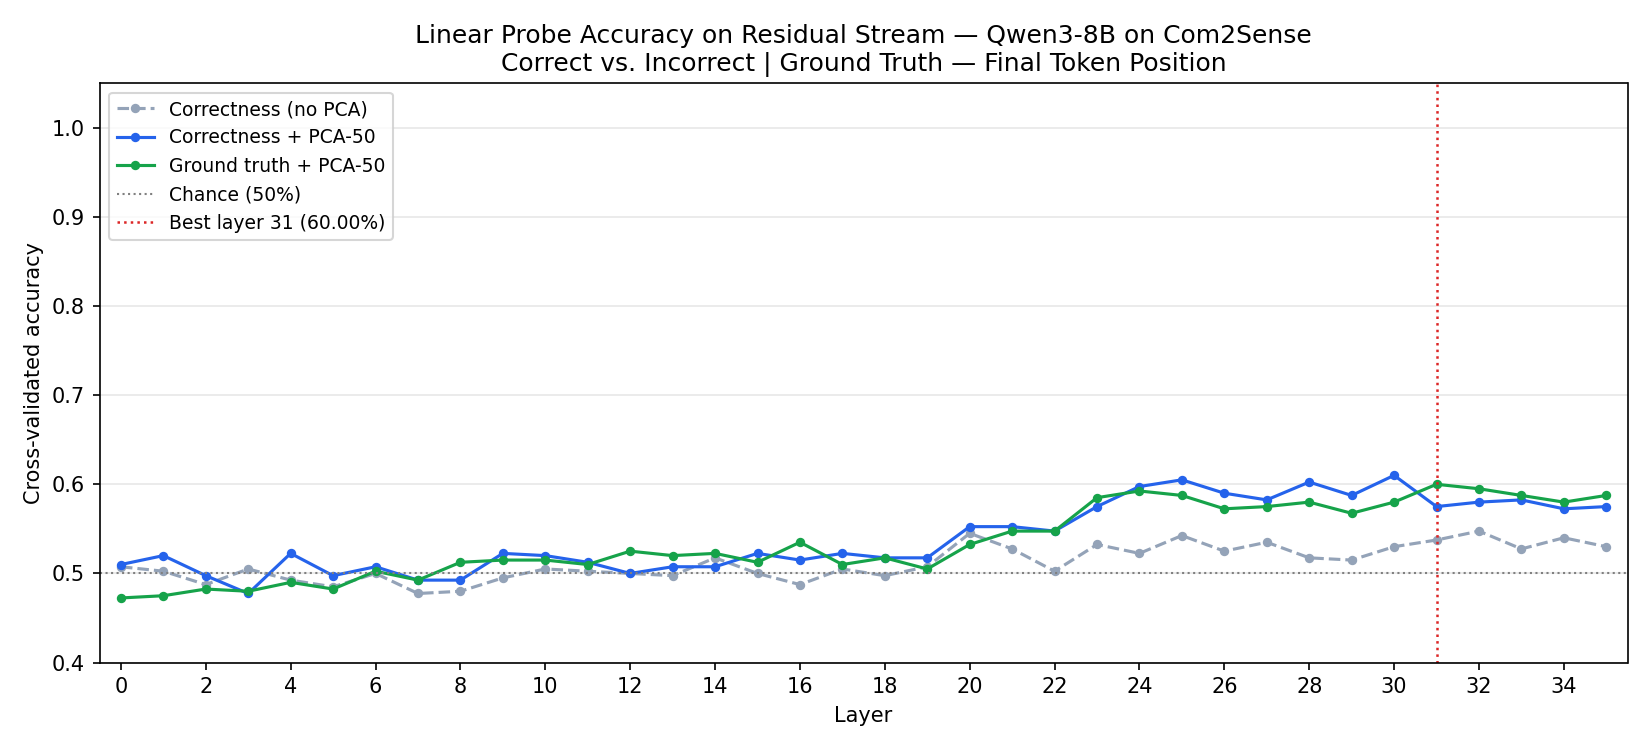
\includegraphics[width=0.48\linewidth]{reports/figures/probe_accuracy_curve.png}
\hfill
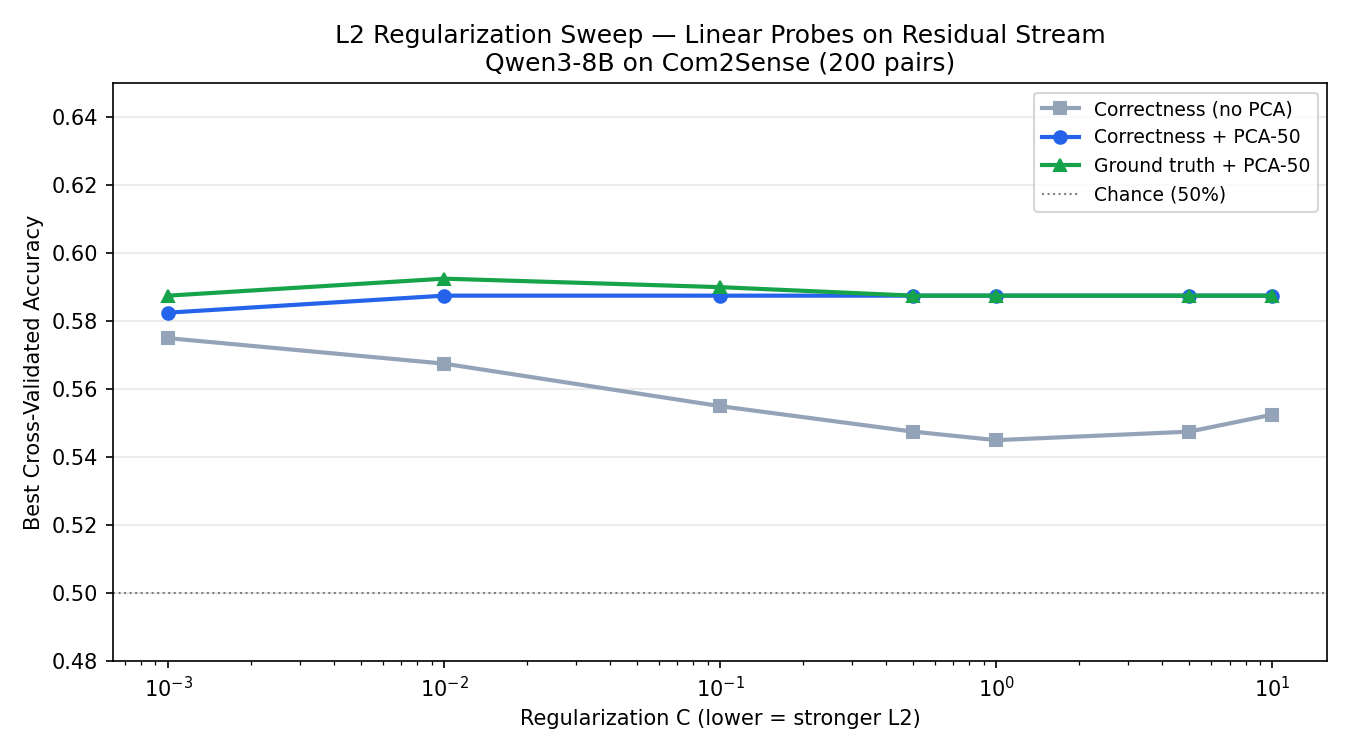
\includegraphics[width=0.48\linewidth]{reports/figures/l2_sweep_results.png}
\caption{\textbf{Left:} Per-layer probing accuracy for three probe configurations. Signal rises from layer 20 and peaks around layer 30. \textbf{Right:} $L_2$ regularization sweep showing corrected accuracies. Overfitting at $C=1$ drops to $\sim$59\% at optimal $C$.}
\label{fig:probing}
\label{fig:l2sweep}
\end{figure}

\subsection{Activation Patching (Phase 3)}

Figure~\ref{fig:patching} shows layer-level activation patching results. Across all 18 layers, the \textbf{prediction flip rate is 0\%}—replacing the incorrect example's full residual stream with the correct example's at any single layer never repairs the prediction. Moreover, all logit changes are negative (mean $\Delta\text{logit}$ ranges from $-0.006$ at layer 18 to $-0.355$ at layer 35), meaning patching consistently \emph{degrades} performance. This monotonically worsening effect is an artifact of distributional mismatch: replacing the entire post-layer state compounds errors across all subsequent layers.

\begin{figure}[t]
\centering
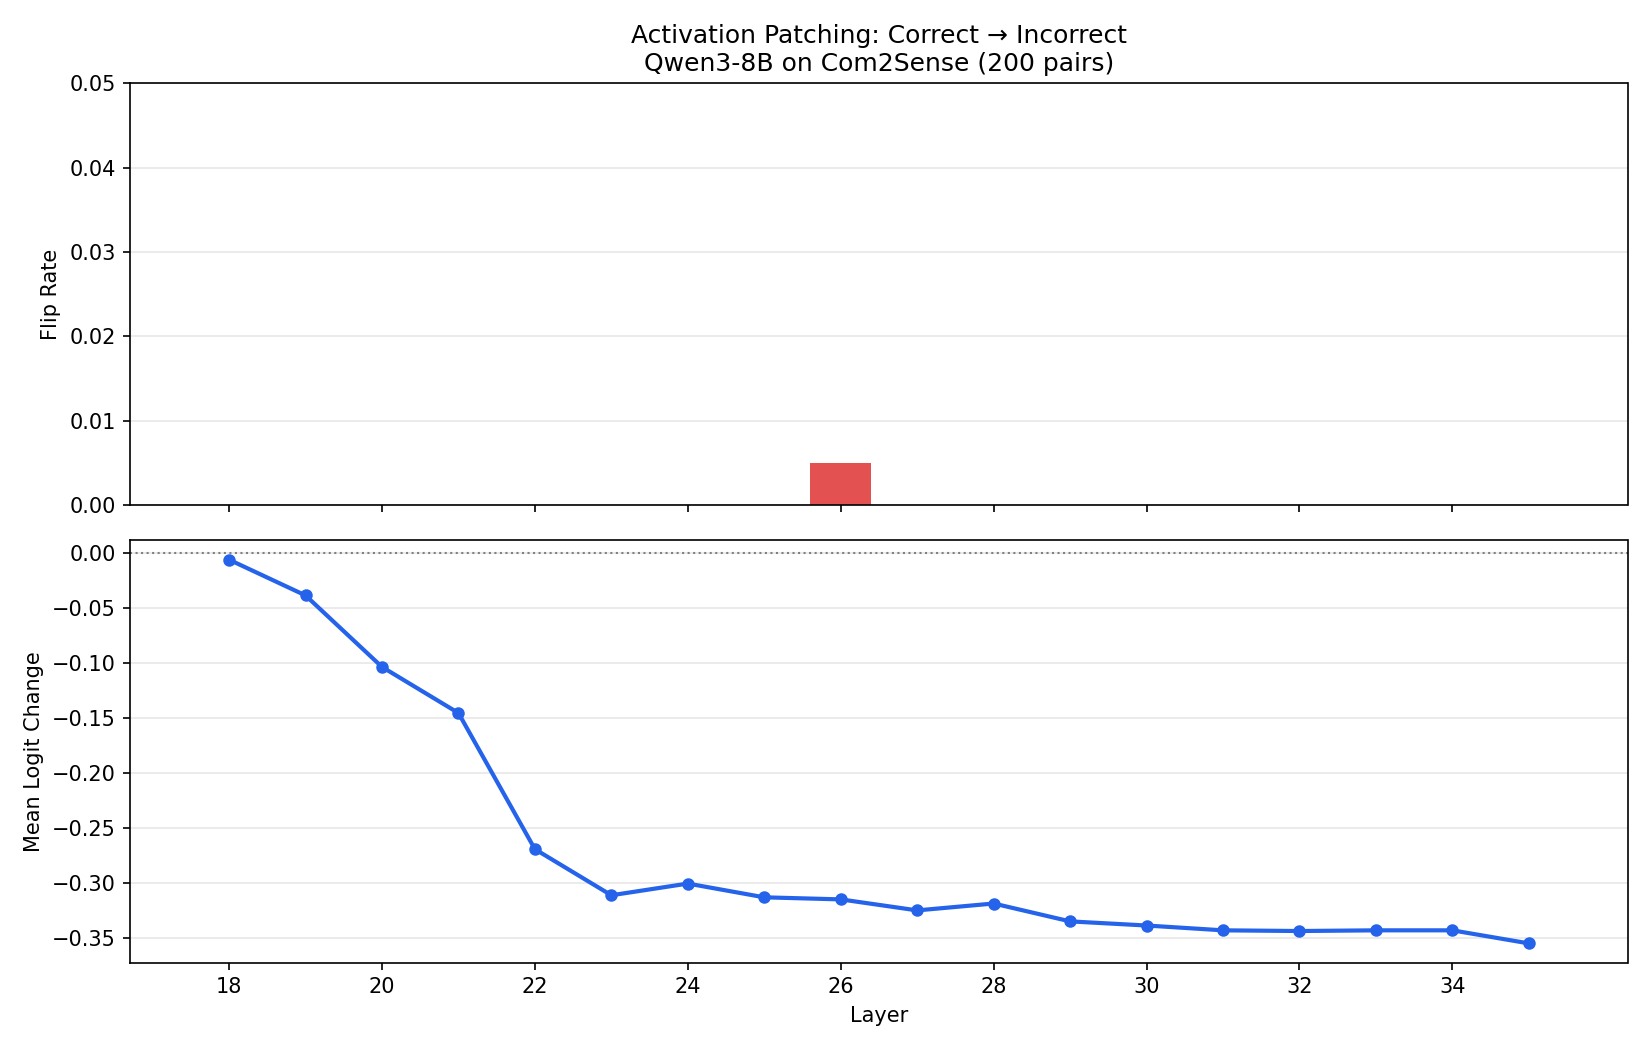
\includegraphics[width=\linewidth]{reports/figures/patching_results.png}
\caption{Layer-level activation patching results. Flip rate is 0\% at all 18 layers; logit change is uniformly negative and grows in magnitude with depth, indicating distributional mismatch from full-stream replacement.}
\label{fig:patching}
\end{figure}

\subsection{Head-Level Analysis (Phase 3)}

\paragraph{Head patching.} Figure~\ref{fig:head_patching} shows the top-10 attention heads by mean patching effect. The most influential head (L20.H8) moves the logit by 0.147 on average—negligible compared to the mean correct-incorrect gap of 2.534. No head produces any prediction flips. The top heads by patching effect cluster in layers 18--26, consistent with the probing results showing signal emerging in this range.

\paragraph{Head probing.} Figure~\ref{fig:head_probe} shows the layer $\times$ head accuracy heatmap. Individual heads match full-stream accuracy: the best head (L32.H20) achieves 59.50\%, nearly identical to the full residual-stream probe (59.25\%). No head stands out; the top-performing heads are spread across layers 28--35 with accuracies tightly clustered at 59--59.5\%.

\paragraph{Ablation.} Mean-ablating each of the 17 candidate heads on 200 correct examples yields a maximum flip rate of \textbf{1.0\%} (L26.H25, 2 flips) and maximum logit change of $|0.028|$. No head is necessary for correct commonsense predictions.

\begin{figure}[t]
\centering
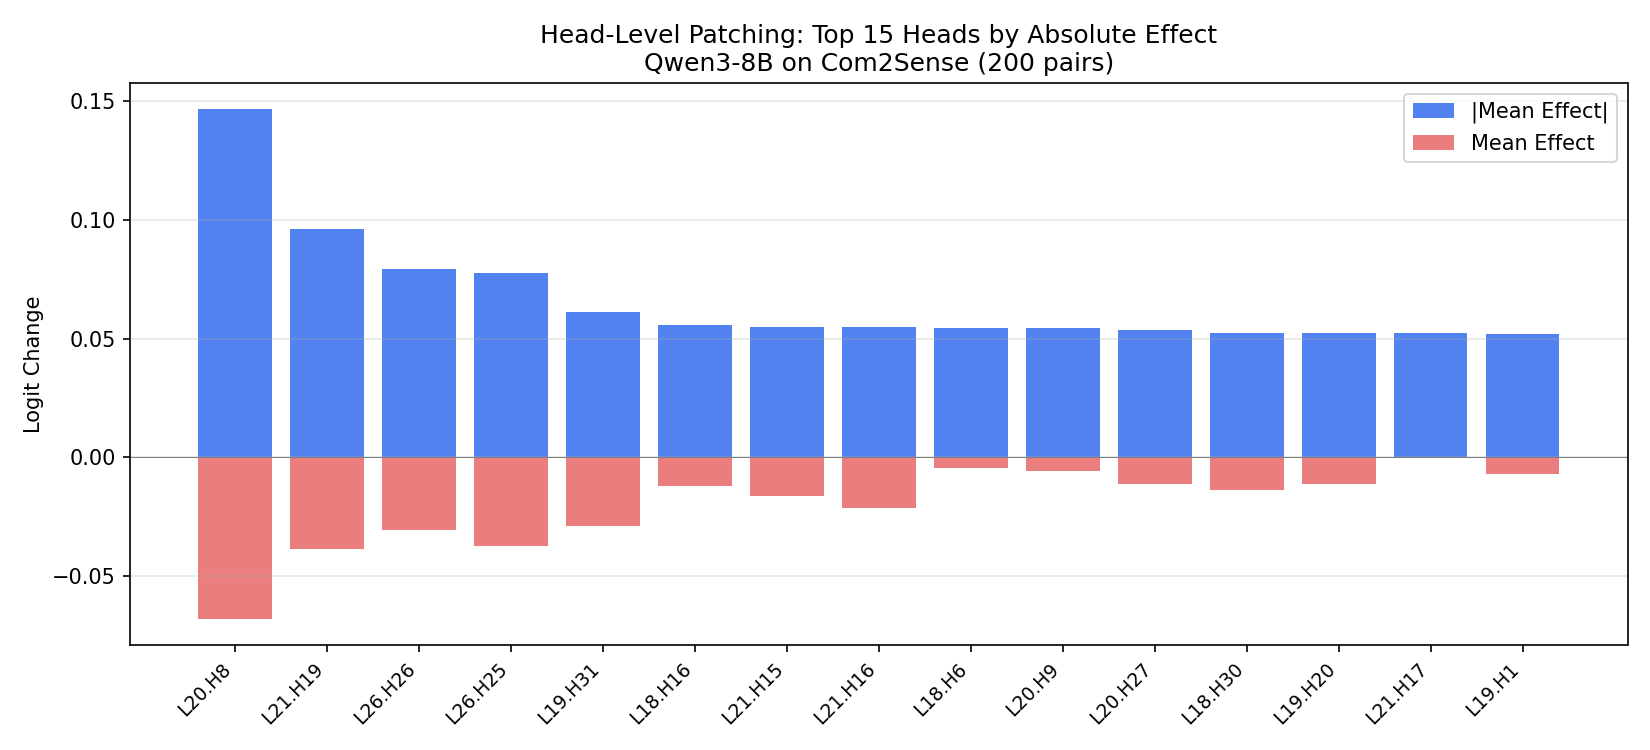
\includegraphics[width=0.48\linewidth]{reports/figures/head_patching_results.png}
\hfill
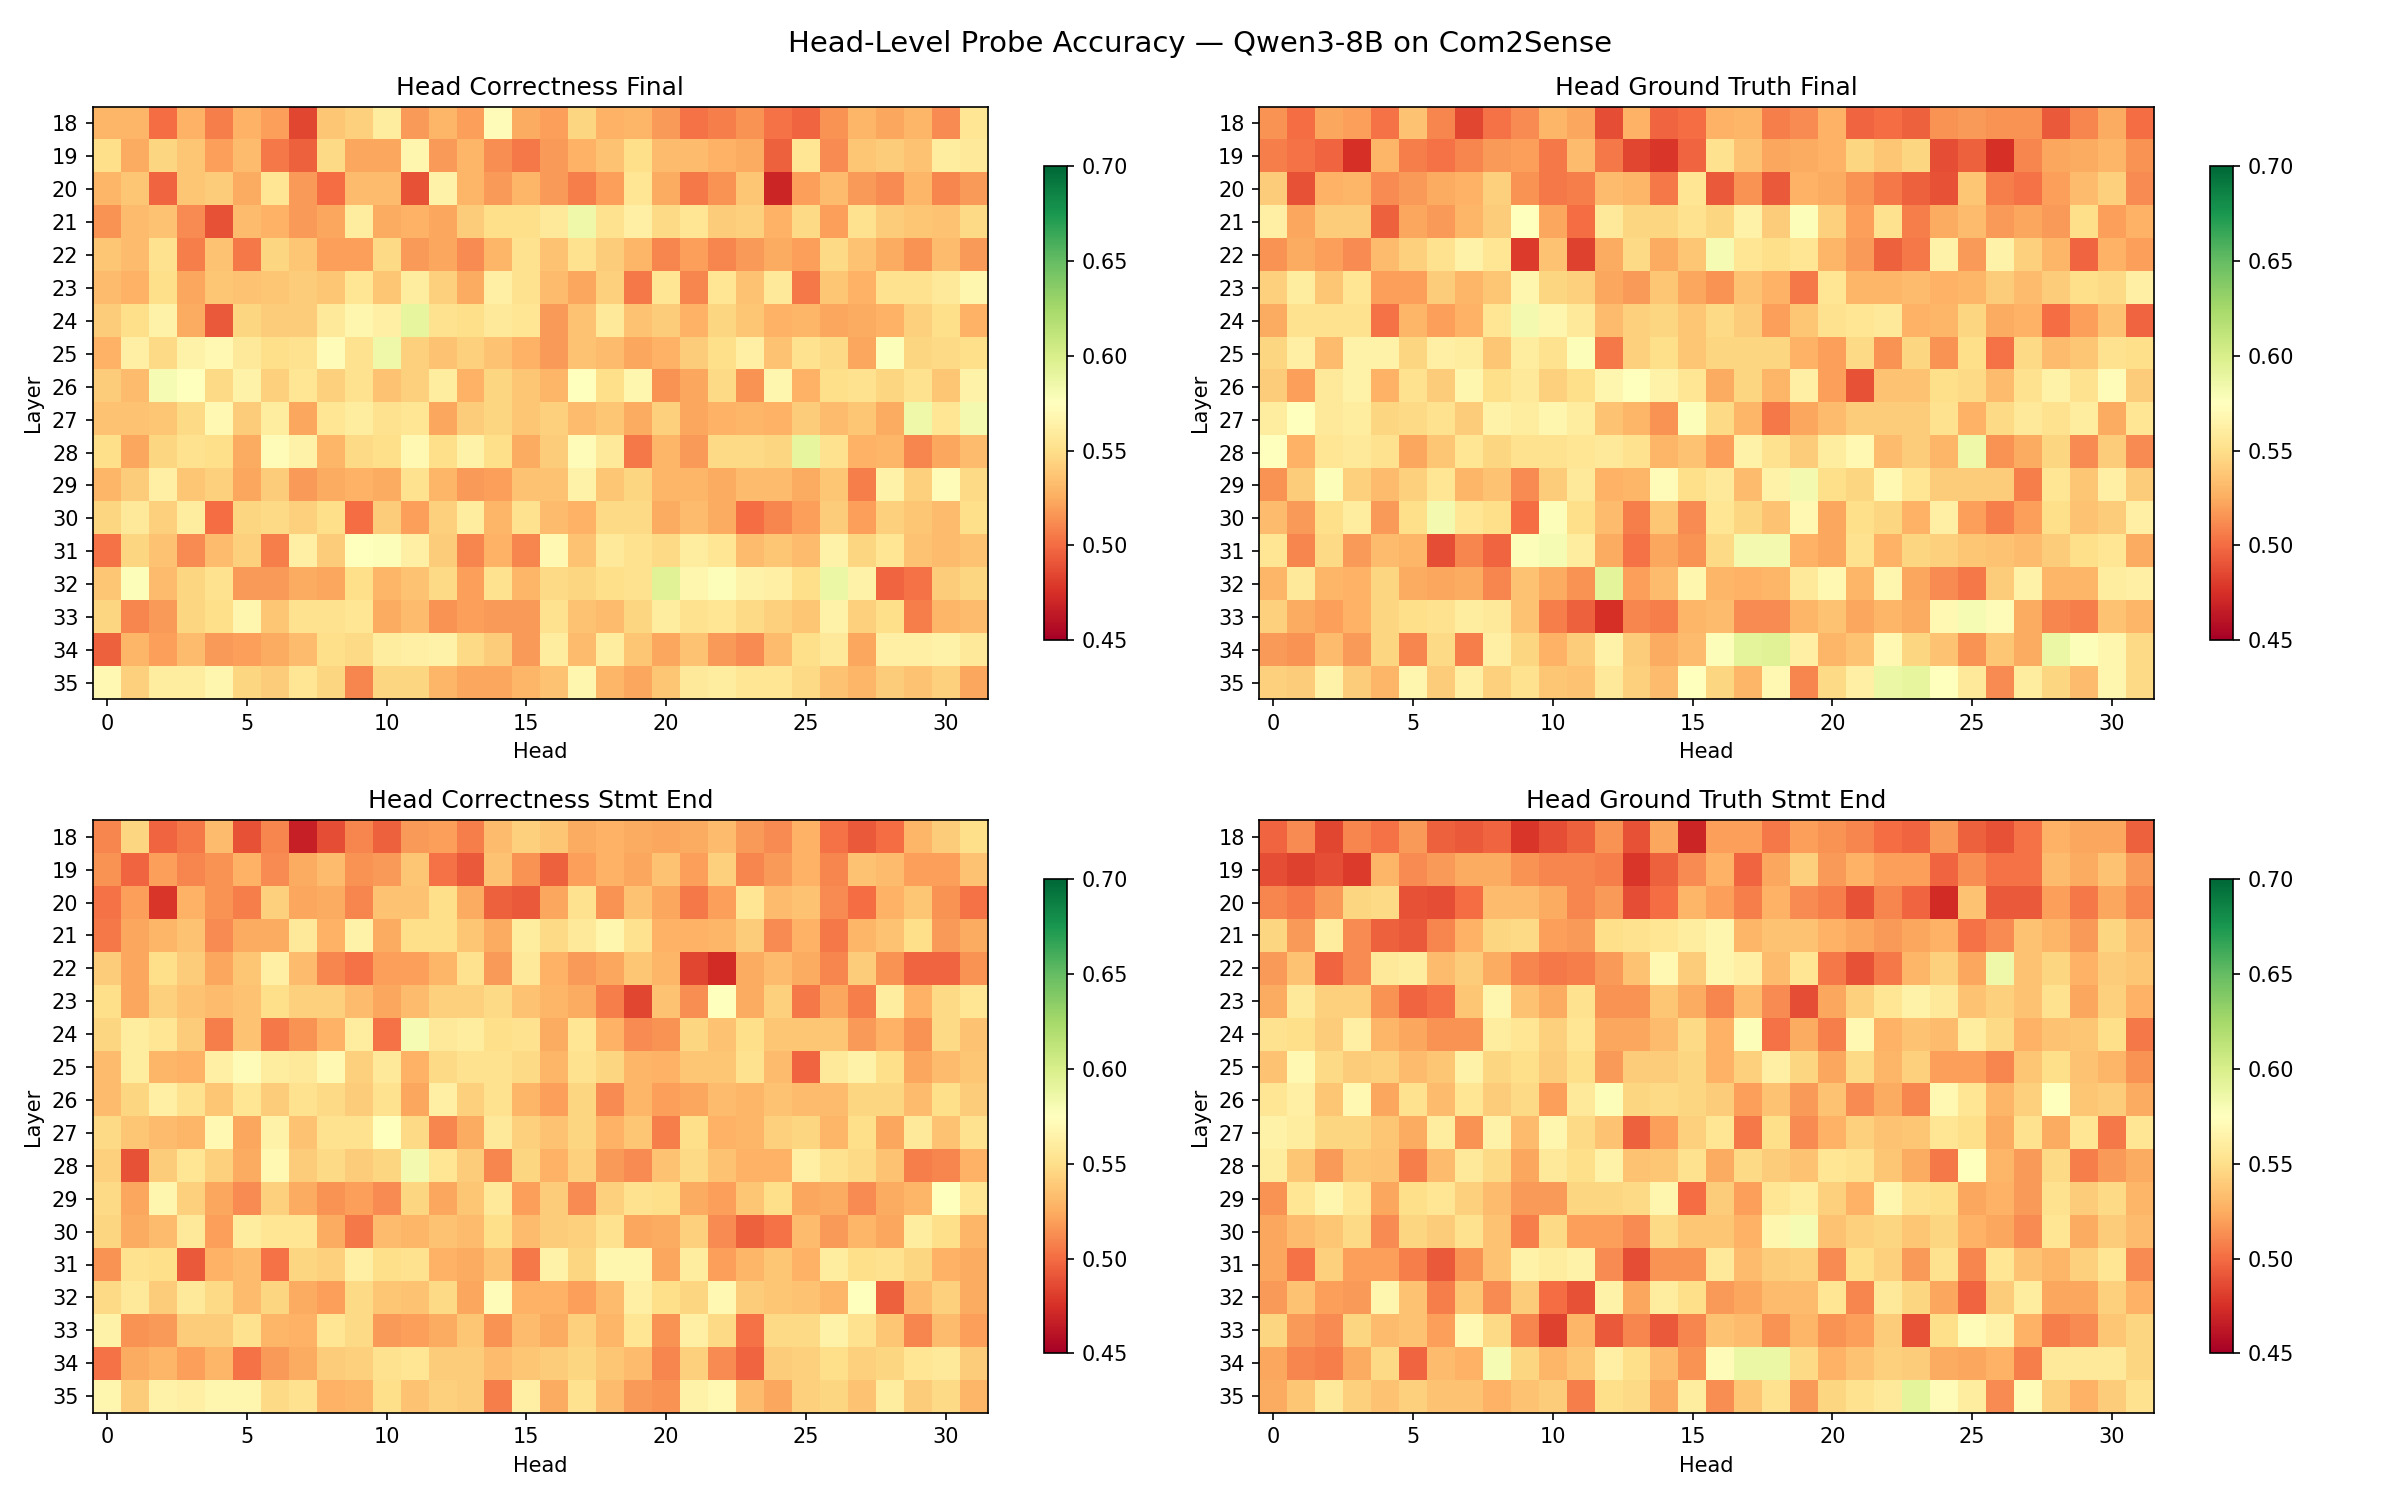
\includegraphics[width=0.48\linewidth]{reports/figures/head_probe_heatmap.png}
\caption{\textbf{Left:} Top attention heads by mean patching effect. Maximum effect is 0.147 (L20.H8); no head produces prediction flips. \textbf{Right:} Layer $\times$ head probing accuracy heatmap. Best individual head (59.5\%) matches full-stream accuracy, indicating distributed encoding.}
\label{fig:head_patching}
\label{fig:head_probe}
\end{figure}

\subsection{Logit Lens Analysis (Phase 4)}

Figure~\ref{fig:logit_lens} shows aggregate logit-lens trajectories for correct (green) and incorrect (red) examples. The trajectories are strikingly symmetric and non-monotonic:

\begin{enumerate}
    \item \textbf{Early divergence}: Correct and incorrect trajectories start separated from layer 0 ($+0.97$ vs.\ $-0.97$).
    \item \textbf{Mid-layer convergence}: Both trajectories partially reverse toward zero in layers 5--19.
    \item \textbf{Late amplification}: Trajectories re-diverge sharply from layer 20, reaching $\pm11$ at layer 30 before settling to $\pm2.5$ at the final layer.
\end{enumerate}

\paragraph{Failure timing.} Among 200 incorrect examples, \textbf{76.5\% are already directionally wrong at layer 0} (i.e., the signed gap is negative from the first measured layer). The mean ``first wrong layer'' is 1.61, and the mean ``stable wrong layer'' (where the wrong-answer bias becomes sustained) is 19.9—matching the layer range where probing first detects signal. Table~\ref{tab:logit_lens_timing} summarizes these statistics.

\begin{table}[t]
\centering
\small
\caption{Logit-lens failure timing statistics across 200 incorrect examples.}
\label{tab:logit_lens_timing}
\begin{tabular}{lc}
\toprule
\textbf{Metric} & \textbf{Value} \\
\midrule
Wrong at layer 0 & 76.5\% (153/200) \\
Mean first-wrong layer & 1.61 \\
Mean stable-wrong layer & 19.9 \\
Mean final gap (correct) & $+2.81$ \\
Mean final gap (incorrect) & $-2.53$ \\
\midrule
\multicolumn{2}{l}{\textit{Final gap by domain (incorrect examples):}} \\
Social & $-3.52$ \\
Temporal & $-2.30$ \\
Time & $-2.20$ \\
\bottomrule
\end{tabular}
\end{table}

\begin{figure}[t]
\centering
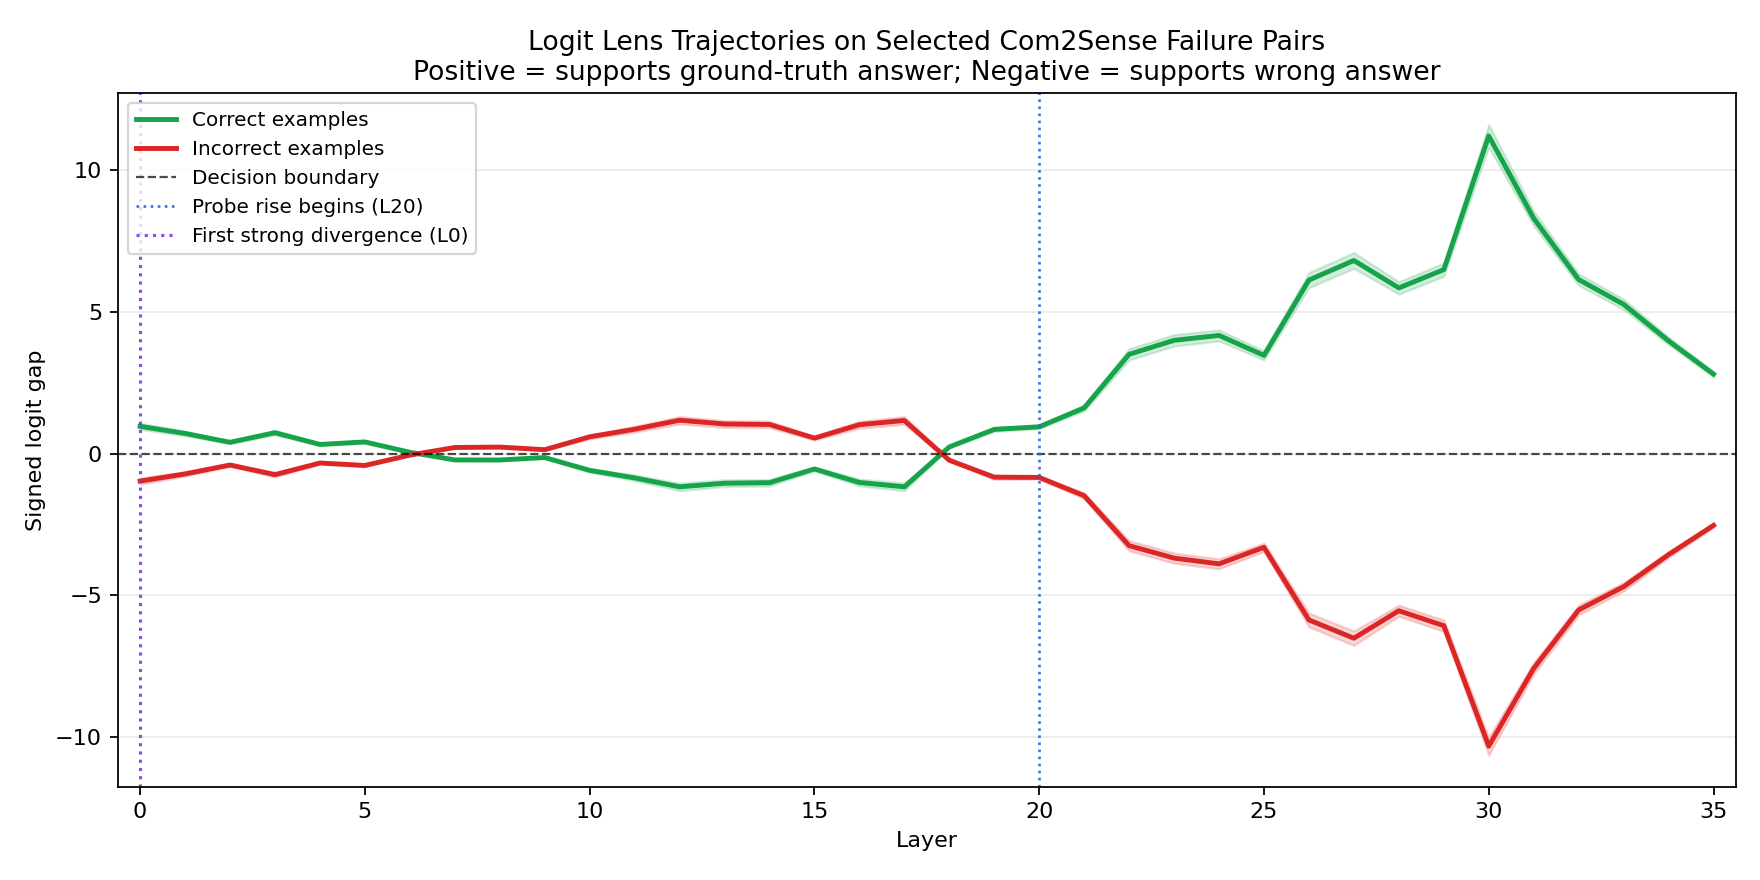
\includegraphics[width=0.55\linewidth]{reports/figures/logit_lens_trajectories.png}
\hfill
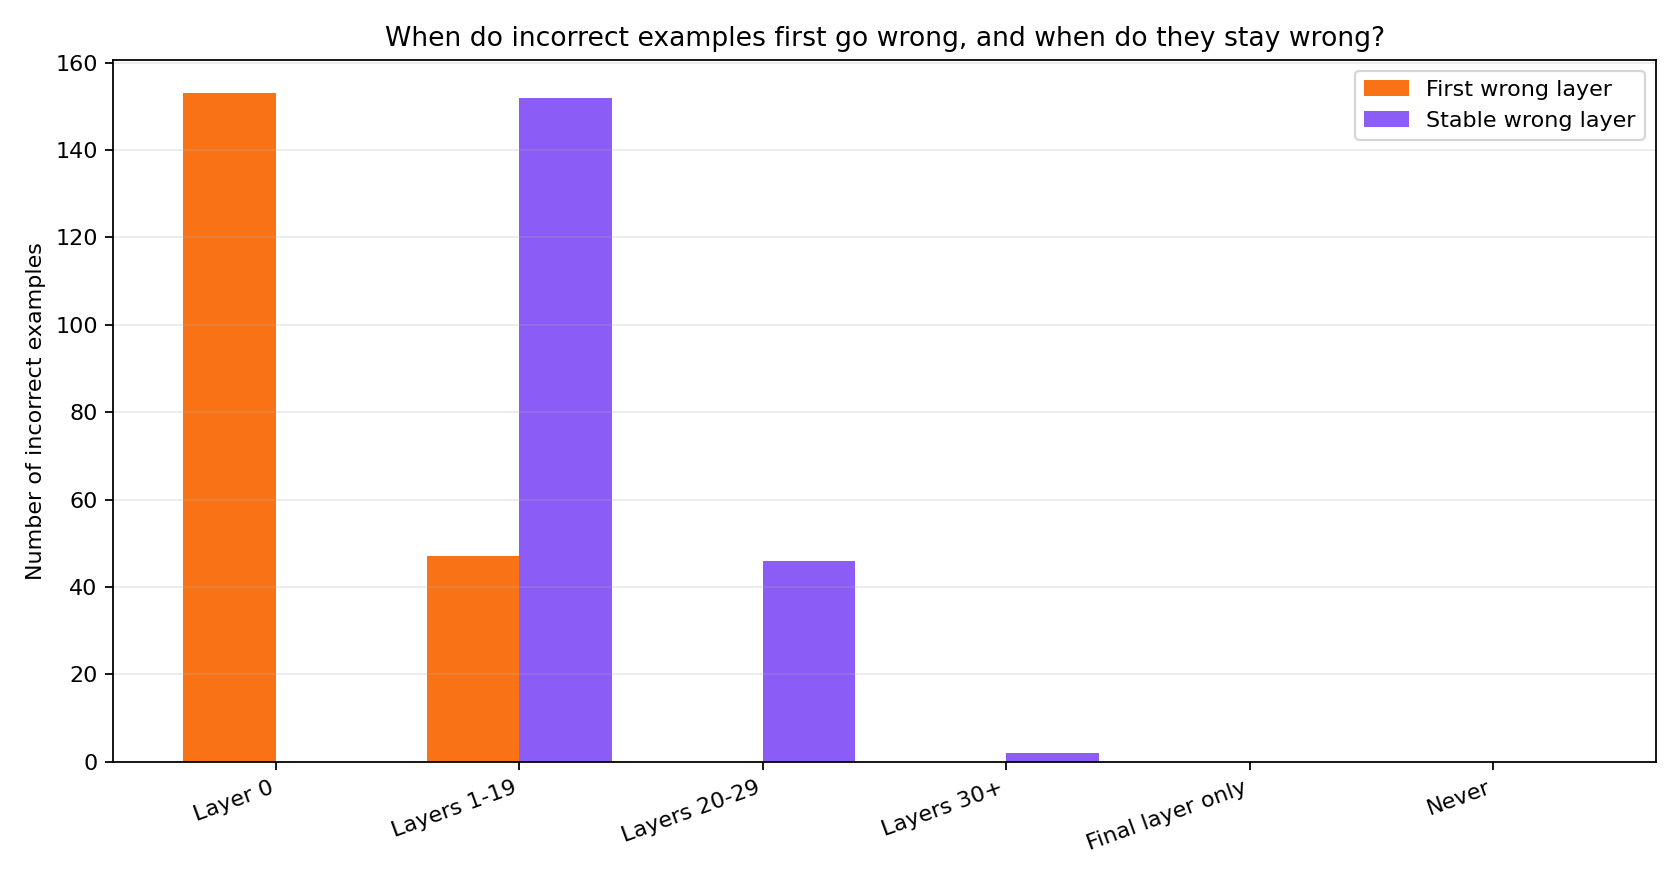
\includegraphics[width=0.42\linewidth]{reports/figures/logit_lens_failure_layers.png}
\caption{\textbf{Left:} Aggregate logit-lens trajectories. Signed logit gap (positive = supports ground truth) for correct (green) and incorrect (red) examples across 36 layers. Trajectories diverge at layer 0, partially converge through mid-layers, then re-diverge strongly from layer 20. \textbf{Right:} Distribution of first-wrong (orange) and stable-wrong (blue) layers for incorrect examples.}
\label{fig:logit_lens}
\end{figure}

\subsection{MLP vs.\ Attention Sublayer Patching (Phase 5)}

Figure~\ref{fig:sublayer} shows results from patching \texttt{hook\_attn\_out} and \texttt{hook\_mlp\_out} separately. Unlike full \texttt{resid\_post} patching (uniformly negative), sublayer patching shows \emph{mixed signs}—some layers produce positive logit changes, others negative. This sign variability reveals that the monotonically negative \texttt{resid\_post} results were an artifact of compounding distributional mismatch, not evidence of causal importance.

\paragraph{Neither sublayer dominates.} The only prediction flips occur at:
\begin{itemize}
    \item \textbf{L25 attention}: 1.5\% flip rate, mean $\Delta\text{logit}=+0.163$ (largest positive intervention)
    \item \textbf{L35 MLP}: 1.5\% flip rate, mean $\Delta\text{logit}=+0.133$
\end{itemize}
Attention effects are larger in magnitude in middle layers (e.g., L20: attn $-0.081$ vs.\ MLP $-0.014$), while MLP effects match attention only at L22--L23. Neither sublayer provides a reliable causal bottleneck.

\begin{table}[t]
\centering
\small
\caption{Selected sublayer patching results (layers 18--35). Attn = attention, MLP = feed-forward.}
\label{tab:sublayer}
\begin{tabular}{lrrrr}
\toprule
\textbf{Layer} & \textbf{Attn flip\%} & \textbf{Attn $\Delta$logit} & \textbf{MLP flip\%} & \textbf{MLP $\Delta$logit} \\
\midrule
18 & 0.0\% & $-0.011$ & 0.0\% & $-0.003$ \\
20 & 0.0\% & $-0.081$ & 0.0\% & $-0.014$ \\
22 & 0.0\% & $-0.156$ & 0.0\% & $-0.149$ \\
\textbf{25} & \textbf{1.5\%} & $\mathbf{+0.163}$ & 0.0\% & $+0.007$ \\
28 & 0.0\% & $+0.003$ & 0.0\% & $-0.045$ \\
32 & 0.0\% & $-0.011$ & 0.0\% & $-0.012$ \\
\textbf{35} & 0.0\% & $-0.018$ & \textbf{1.5\%} & $\mathbf{+0.133}$ \\
\bottomrule
\end{tabular}
\end{table}

\begin{figure}[t]
\centering
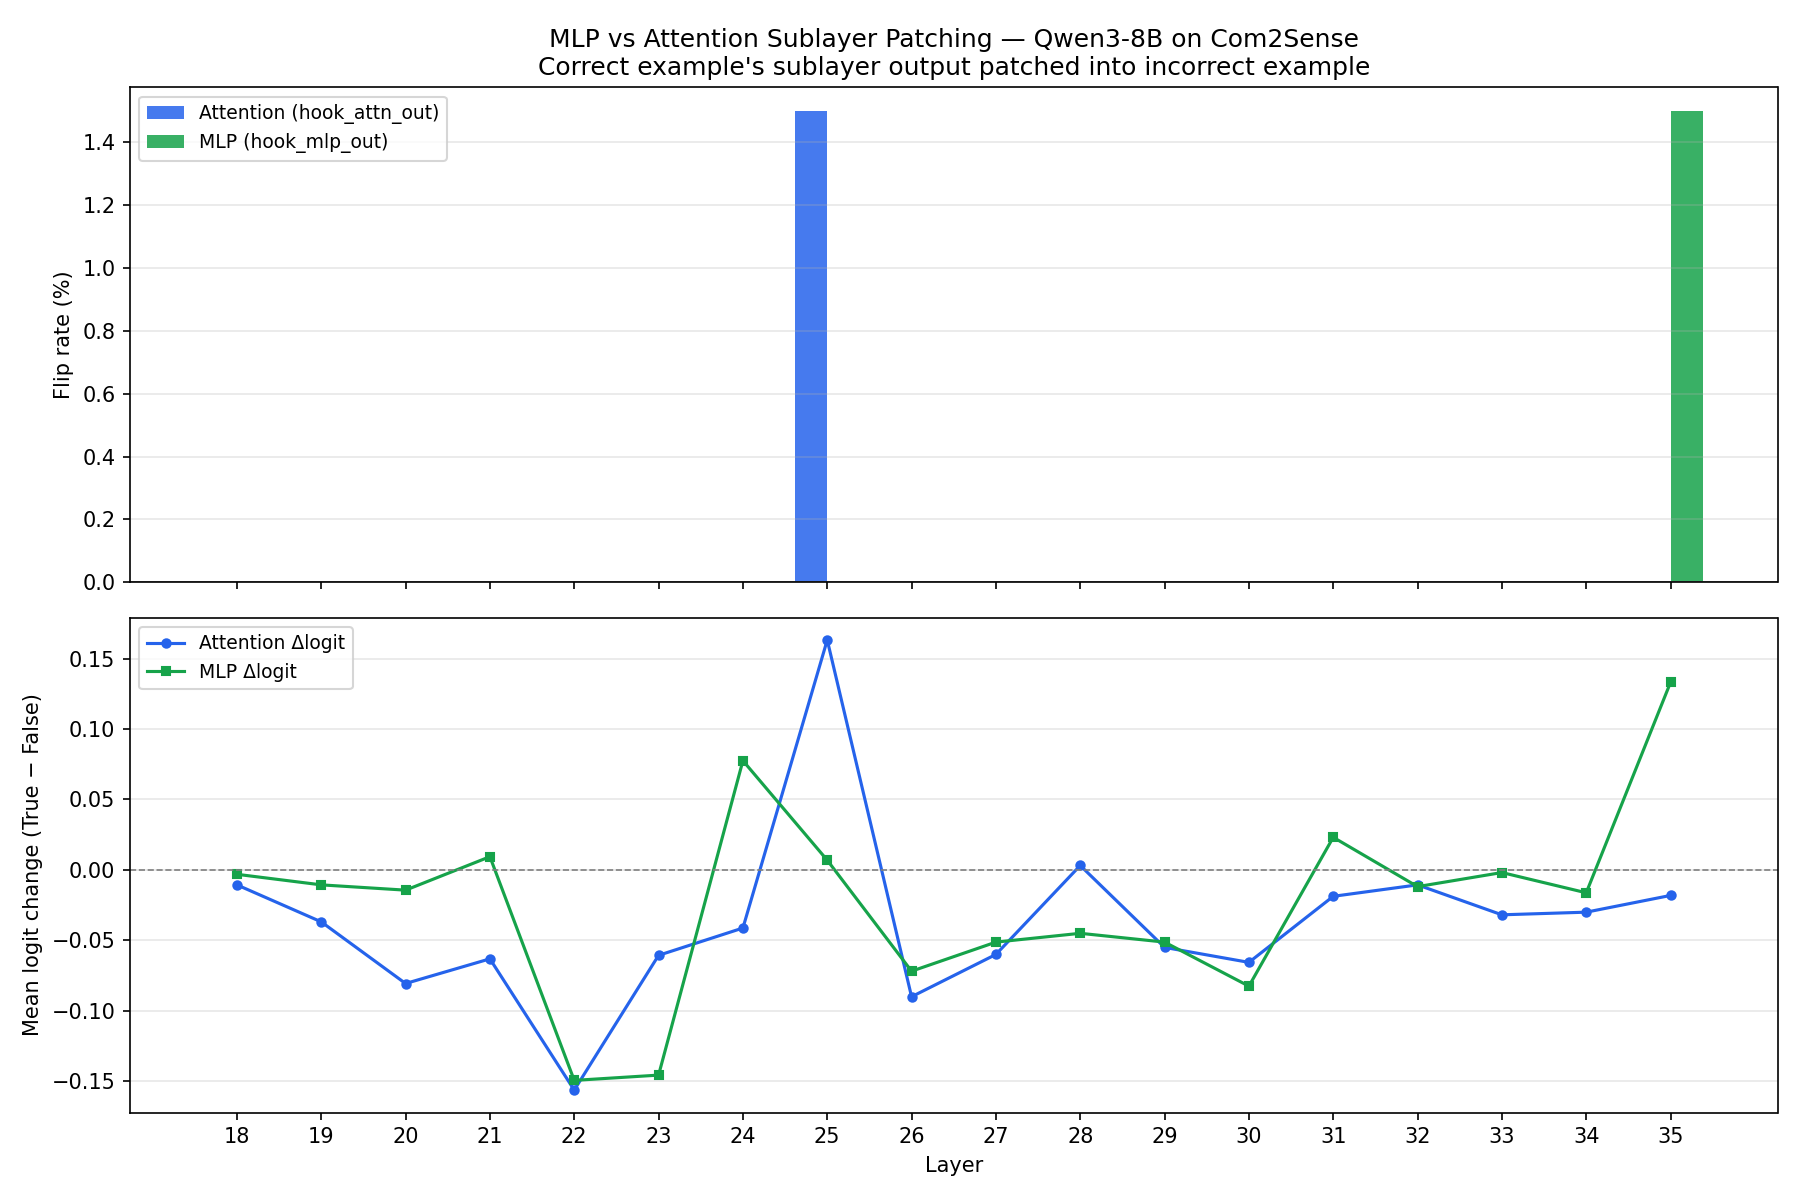
\includegraphics[width=\linewidth]{reports/figures/mlp_attn_patching.png}
\caption{MLP vs.\ attention sublayer patching results. Unlike full-stream patching (Figure~\ref{fig:patching}), sublayer effects have mixed signs. L25 attention is the only intervention producing reliable positive logit shifts (1.5\% flips).}
\label{fig:sublayer}
\end{figure}

\section{Discussion}
\label{sec:discussion}

\subsection{Answers to Research Questions}

\paragraph{Q1: Localized or distributed?}
\textbf{Distributed.} The convergent evidence across all experiments points to distribution: 0\% flip rates from layer patching and head patching, 1.5\% maximum from sublayer patching, 1.0\% maximum from ablation, and per-head probing that matches full-stream accuracy. No minimal set of components reliably mediates commonsense predictions.

This contrasts markedly with factual recall findings. \citet{geva2023dissecting} report flip rates of 30--60\%+ for factual associations in GPT models. \citet{wang2022interpretability} identify a specific circuit for indirect object identification. Commonsense—with its demand for multi-hop world knowledge integration—does not admit such localization.

\paragraph{Q2: Knowledge-retrieval or inference failure?}
\textbf{Early bias with late consolidation.} Logit-lens analysis reveals a two-stage failure process that refines our initial hypothesis. Before logit-lens, probing suggested a purely late-onset inference failure (signal emerging at layer 20). Logit-lens shows that 76.5\% of incorrect examples are \emph{already} directionally wrong at layer 0—suggesting early representational bias—but these wrong-direction biases are not stably committed until $\sim$layer 20.

This is inconsistent with either a pure retrieval failure (the model never had the knowledge) or a pure inference failure (wrong computation on correct representations). Instead, the model builds an early weak bias toward the wrong answer, then consolidates it through late-layer computation.

\paragraph{Q3: Attention or MLP?}
\textbf{Neither dominates.} We do not replicate the MLP dominance reported by other teams studying PIQA-style tasks. This may reflect architectural differences (Qwen3-8B uses grouped-query attention, differing from GPT-2) or task differences (Com2Sense requires multi-hop commonsense vs.\ PIQA's single-step physical intuition). The single most helpful intervention—L25 attention, $+0.163$ logit change, 1.5\% flips—suggests attention may play a slightly more facilitative role in late-layer reasoning, but the effect is too small to be diagnostically useful.

\subsection{Implications}

\paragraph{Surgical repair is ineffective.}
Given that no single component is sufficient or necessary, targeted patching cannot repair commonsense failures in the way it can for factual recall. Commonsense failures require understanding and addressing the underlying \emph{representational} weakness ($\sim$59\% probing accuracy) rather than a specific computational bottleneck.

\paragraph{Two-stage model.}
Our findings suggest a revised model of commonsense failure: an \emph{early-bias, late-consolidation} mechanism where initial directional biases (possibly reflecting training data priors, e.g., the observed false-bias) are amplified by late-layer computation. The reversal and re-divergence of logit-lens trajectories (Figure~\ref{fig:logit_lens}) suggests the network iteratively revises its judgment rather than computing it at a single location.

\paragraph{Implications for alignment.}
If commonsense failures are distributed and representationally diffuse, they cannot be patched by localizing and editing specific circuits. This suggests that improving commonsense reliability likely requires changes to the training distribution—specifically, more high-quality commonsense examples that build stronger representational encodings—rather than post-hoc surgical intervention.

\subsection{Limitations}

This study is limited to a single model (Qwen3-8B) and single dataset (Com2Sense). The 200-pair subset, while sufficient for reliable statistical patterns, may not capture all failure modes. Probing accuracy of $\sim$59\% is real but weak—stronger probes (e.g., nonlinear, token-averaged) might reveal more structure. We do not ablate full attention layers or MLP blocks, only individual heads; block-level ablation might reveal stronger effects. Causal attribution from activation patching is limited by distributional mismatch between different input sentences; techniques like path patching~\citep{conmy2023towards} that control for this mismatch could reveal additional structure.

\section{Conclusion}
\label{sec:conclusion}

We have presented a systematic mechanistic interpretability study of commonsense reasoning failures in Qwen3-8B, combining five complementary techniques across 200 asymmetric complementary pairs from Com2Sense. Our central finding is that commonsense failures are \emph{distributed}: no single layer, attention head, or sublayer is sufficient (0\% flip rates) or necessary (max 1\% flip rates) for correct commonsense predictions. Logit-lens analysis reveals that failures involve an early representational bias (76.5\% of incorrect examples are wrong-directional from layer 0) that consolidates and amplifies in the model's second half (layers 20--35). Probing accuracy plateaus at $\sim$59\%, indicating weak but genuine signal that is spread redundantly across the residual stream.

These findings challenge the assumption that commonsense failures can be diagnosed and repaired through the same localized circuit-finding methodology that has proven successful for factual recall. Commonsense failures appear to require a different treatment: strengthening the underlying representational encoding through training, rather than patching specific computational components after the fact.

\section*{Author Contributions}
All authors contributed equally to experimental design, implementation, and analysis.

\section*{Acknowledgments}
We thank the TransformerLens team for their interpretability toolkit and Modal for providing GPU compute infrastructure. Evaluation and analysis were conducted on A100-80GB GPUs.

\bibliography{paper}
\bibliographystyle{colm2026_conference}

\appendix
\section{Additional Figures}
\label{app:figures}

\begin{figure}[h]
\centering
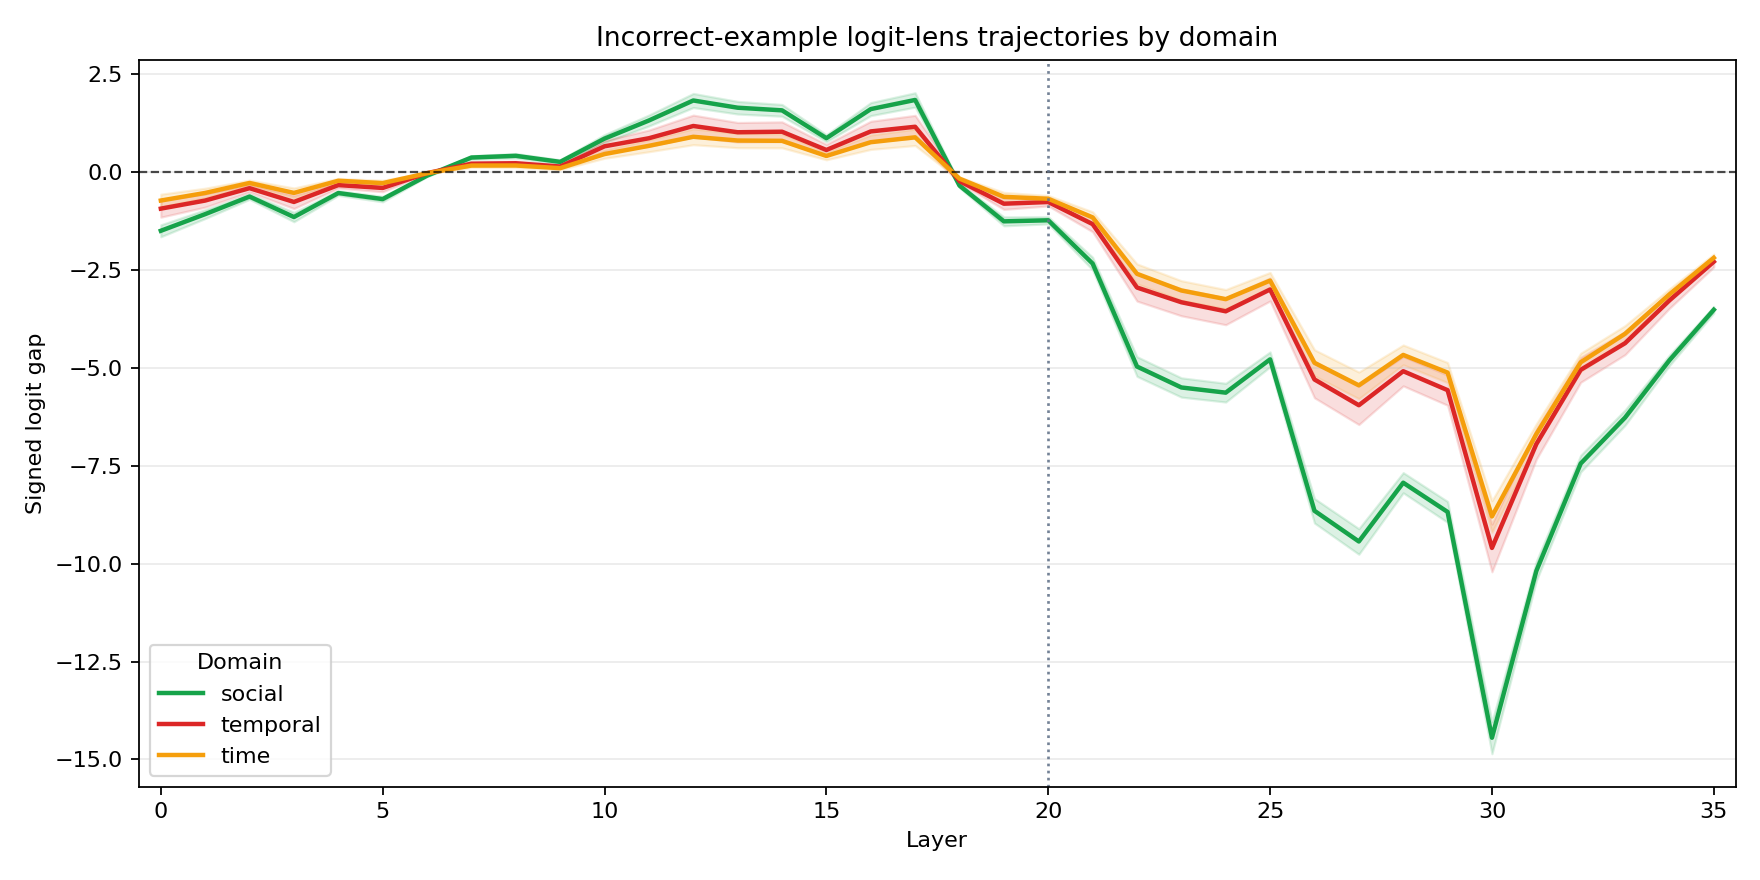
\includegraphics[width=\linewidth]{reports/figures/logit_lens_domain_trajectories.png}
\caption{Logit-lens trajectories broken down by domain (physical, social, temporal, time) for incorrect examples. Social failures show the most extreme final signed gap ($-3.52$), while temporal failures show the weakest ($-2.30$).}
\label{fig:domain_trajectories}
\end{figure}

\begin{figure}[h]
\centering
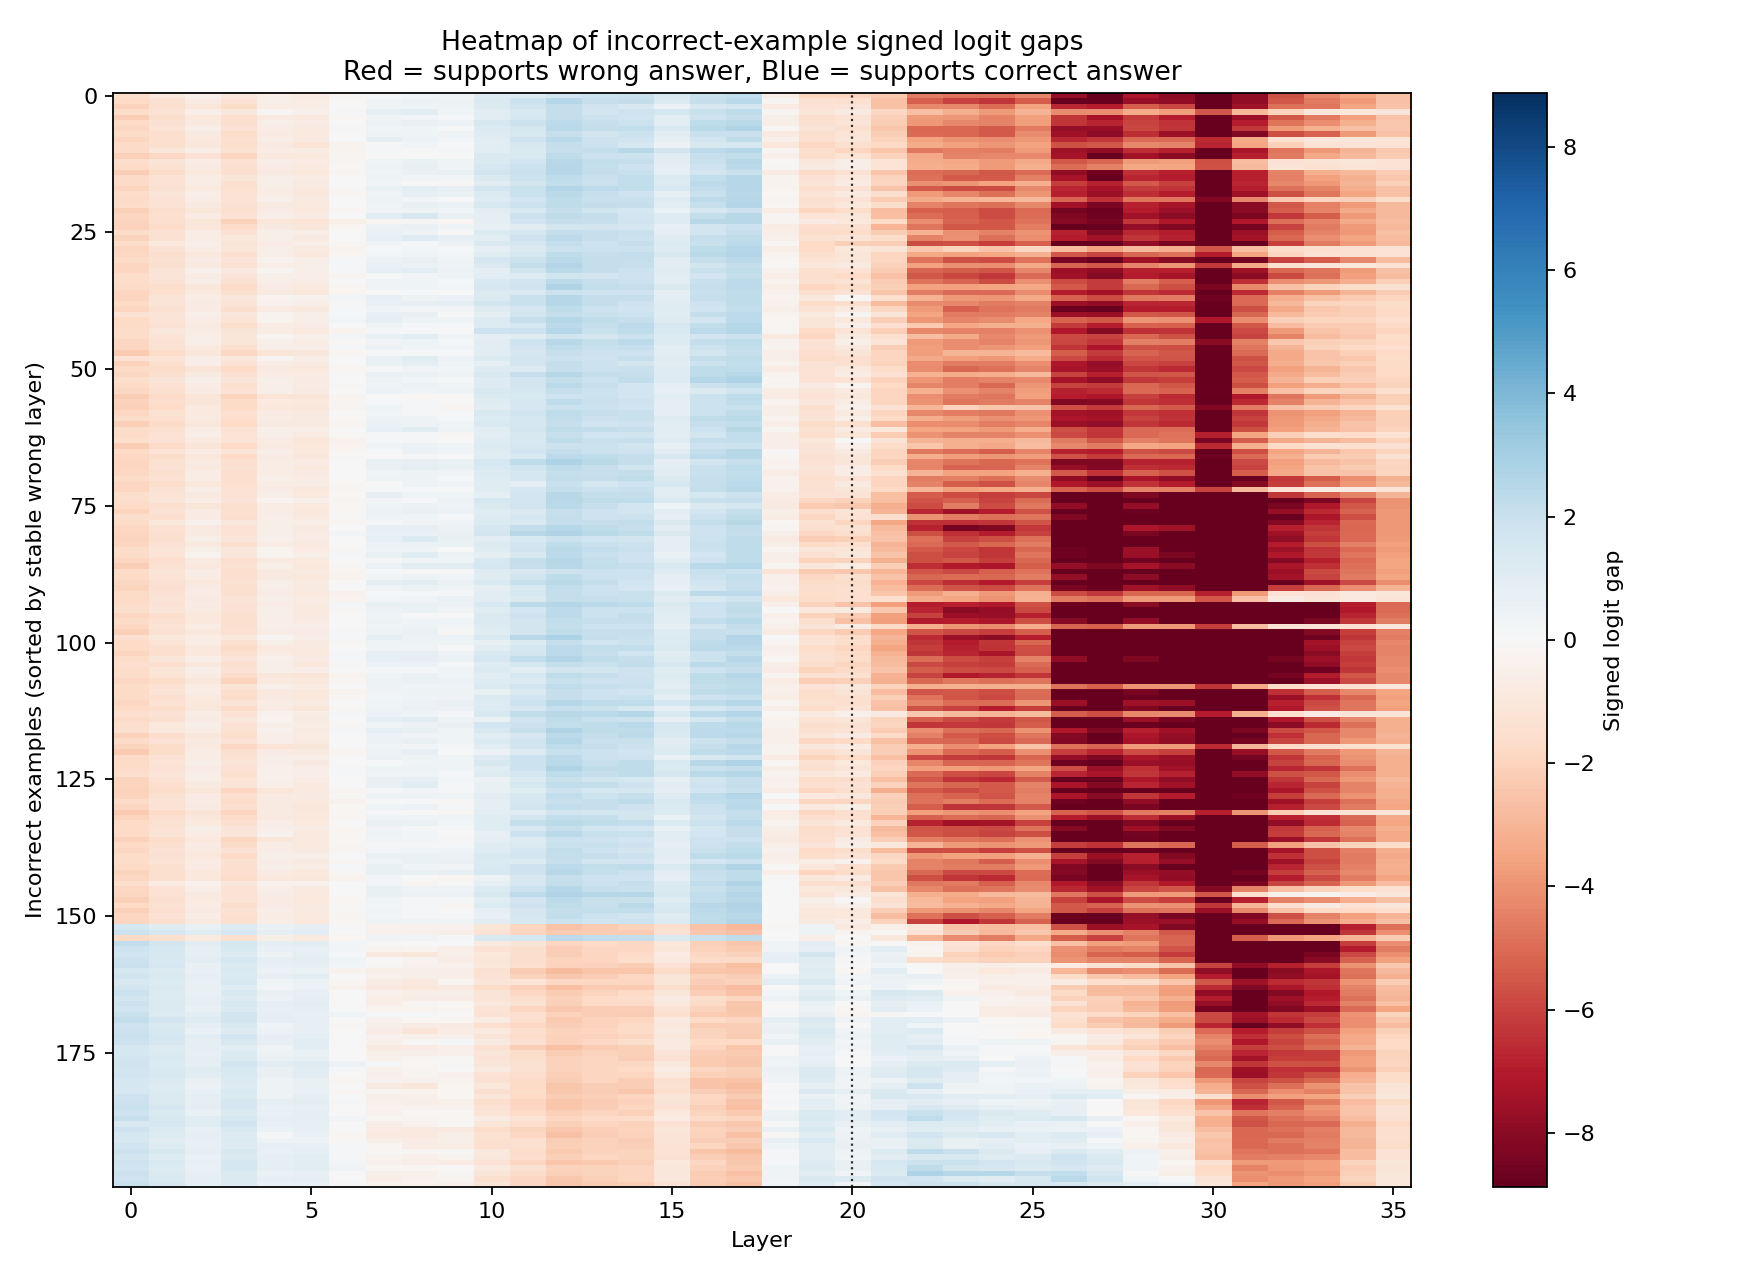
\includegraphics[width=\linewidth]{reports/figures/logit_lens_incorrect_heatmap.png}
\caption{Heatmap of signed logit gaps for all 200 incorrect examples across 36 layers. Rows are examples, columns are layers. Most examples are red (wrong direction) from early layers; a minority start blue and turn red around layer 20.}
\label{fig:heatmap}
\end{figure}

\begin{figure}[h]
\centering
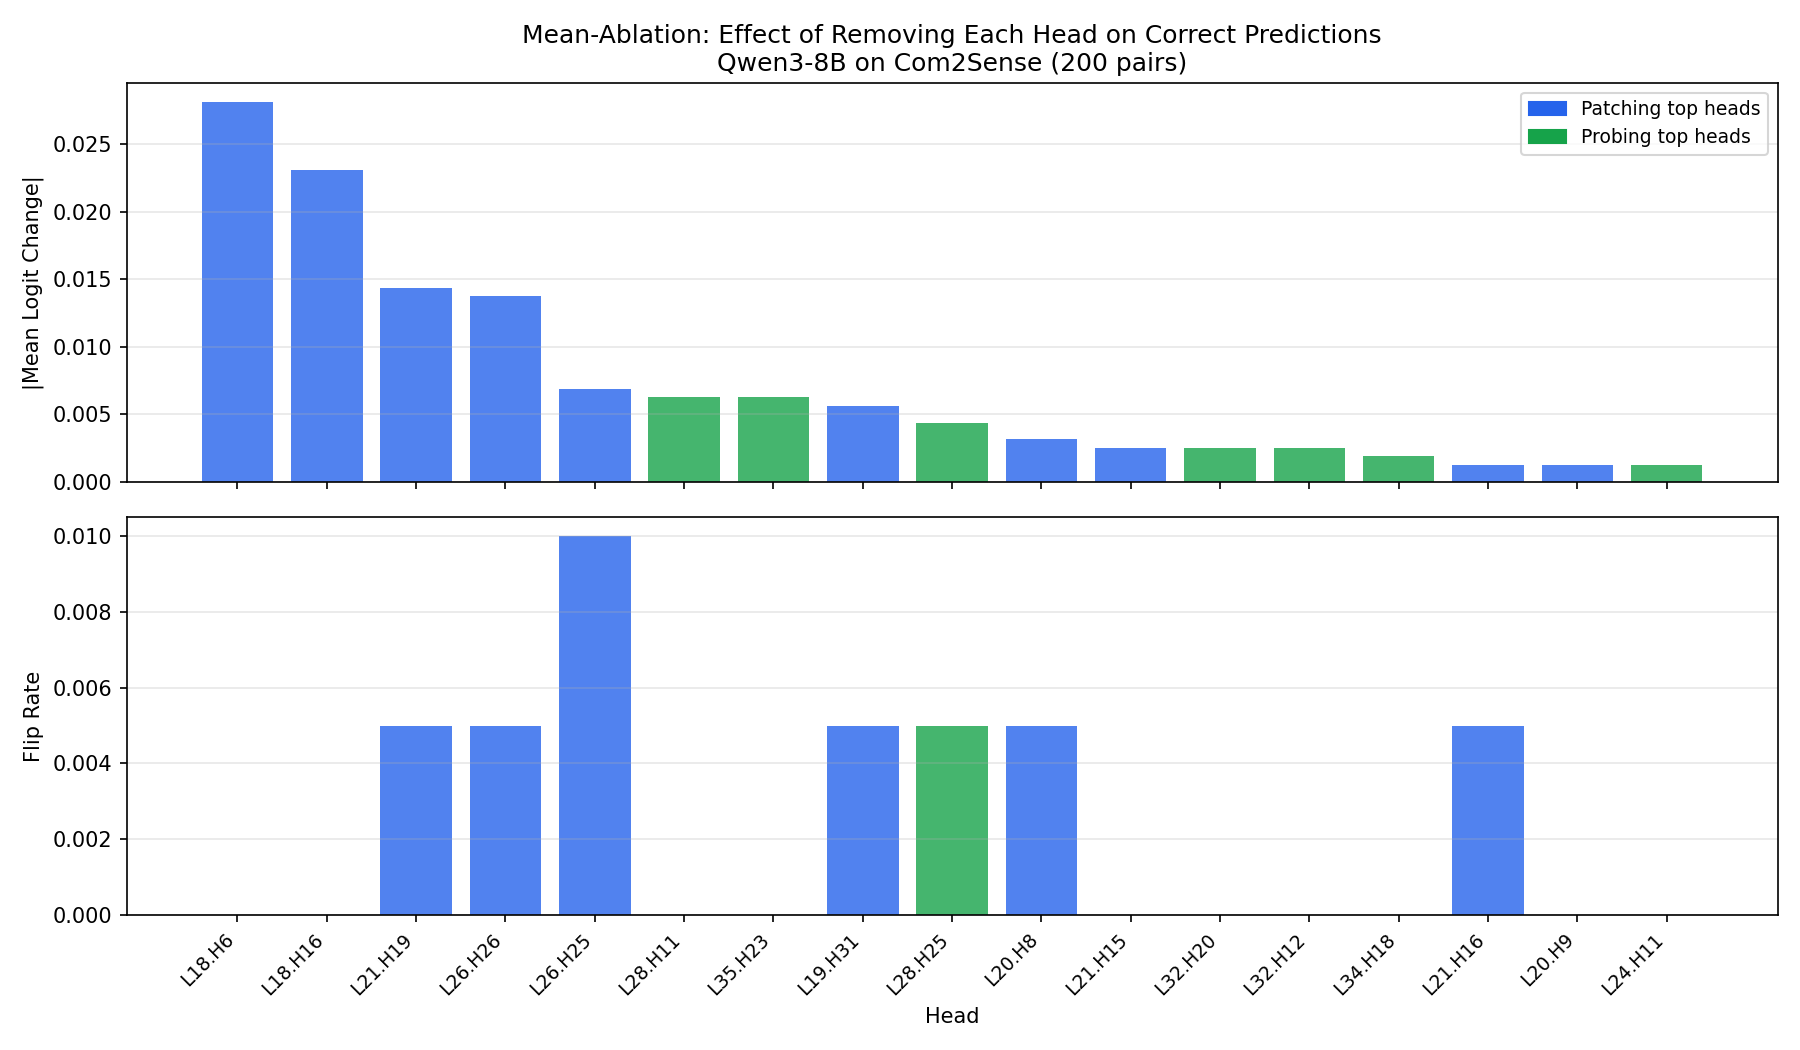
\includegraphics[width=0.75\linewidth]{reports/figures/ablation_results.png}
\caption{Mean-ablation flip rates for 17 candidate attention heads. Maximum flip rate is 1.0\% (L26.H25, 2/200 correct predictions flipped). No head is necessary for commonsense predictions.}
\label{fig:ablation}
\end{figure}

\section{Full Sublayer Patching Results}
\label{app:sublayer}

\begin{table}[h]
\centering
\small
\caption{Complete MLP vs.\ attention sublayer patching results for all 18 layers.}
\label{tab:full_sublayer}
\begin{tabular}{lrrrr}
\toprule
\textbf{Layer} & \textbf{Attn flip\%} & \textbf{Attn $\Delta$logit} & \textbf{MLP flip\%} & \textbf{MLP $\Delta$logit} \\
\midrule
18 & 0.0\% & $-0.011$ & 0.0\% & $-0.003$ \\
19 & 0.0\% & $-0.037$ & 0.0\% & $-0.011$ \\
20 & 0.0\% & $-0.081$ & 0.0\% & $-0.014$ \\
21 & 0.0\% & $-0.063$ & 0.0\% & $+0.009$ \\
22 & 0.0\% & $-0.156$ & 0.0\% & $-0.149$ \\
23 & 0.0\% & $-0.061$ & 0.0\% & $-0.146$ \\
24 & 0.0\% & $-0.041$ & 0.0\% & $+0.077$ \\
25 & 1.5\% & $+0.163$ & 0.0\% & $+0.007$ \\
26 & 0.0\% & $-0.090$ & 0.0\% & $-0.072$ \\
27 & 0.0\% & $-0.060$ & 0.0\% & $-0.051$ \\
28 & 0.0\% & $+0.003$ & 0.0\% & $-0.045$ \\
29 & 0.0\% & $-0.055$ & 0.0\% & $-0.051$ \\
30 & 0.0\% & $-0.066$ & 0.0\% & $-0.083$ \\
31 & 0.0\% & $-0.019$ & 0.0\% & $+0.023$ \\
32 & 0.0\% & $-0.011$ & 0.0\% & $-0.012$ \\
33 & 0.0\% & $-0.032$ & 0.0\% & $-0.002$ \\
34 & 0.0\% & $-0.030$ & 0.0\% & $-0.016$ \\
35 & 0.0\% & $-0.018$ & 1.5\% & $+0.133$ \\
\bottomrule
\end{tabular}
\end{table}

\section{Ablation Study Details}
\label{app:ablation}

\begin{table}[h]
\centering
\small
\caption{Full mean-ablation results for 17 candidate heads.}
\label{tab:ablation}
\begin{tabular}{lrrrrr}
\toprule
\textbf{Head} & \textbf{Flips} & \textbf{Flip\%} & \textbf{Mean $\Delta$logit} & \textbf{Median} & \textbf{Std} \\
\midrule
L26.H25 & 2 & 1.0\% & $+0.007$ & 0.0 & 0.153 \\
L20.H8  & 1 & 0.5\% & $+0.003$ & 0.0 & 0.186 \\
L21.H19 & 1 & 0.5\% & $-0.014$ & 0.0 & 0.126 \\
L26.H26 & 1 & 0.5\% & $+0.014$ & 0.0 & 0.156 \\
L19.H31 & 1 & 0.5\% & $-0.006$ & 0.0 & 0.096 \\
L21.H16 & 1 & 0.5\% & $-0.001$ & 0.0 & 0.084 \\
L28.H25 & 1 & 0.5\% & $-0.004$ & 0.0 & 0.073 \\
L18.H16 & 0 & 0.0\% & $+0.023$ & 0.0 & 0.080 \\
L21.H15 & 0 & 0.0\% & $-0.003$ & 0.0 & 0.098 \\
L18.H6  & 0 & 0.0\% & $+0.028$ & 0.0 & 0.081 \\
L20.H9  & 0 & 0.0\% & $+0.001$ & 0.0 & 0.088 \\
L32.H20 & 0 & 0.0\% & $+0.003$ & 0.0 & 0.067 \\
L34.H18 & 0 & 0.0\% & $+0.002$ & 0.0 & 0.069 \\
L28.H11 & 0 & 0.0\% & $+0.006$ & 0.0 & 0.075 \\
L24.H11 & 0 & 0.0\% & $+0.001$ & 0.0 & 0.078 \\
L32.H12 & 0 & 0.0\% & $+0.003$ & 0.0 & 0.075 \\
L35.H23 & 0 & 0.0\% & $-0.006$ & 0.0 & 0.073 \\
\bottomrule
\end{tabular}
\end{table}

\end{document}
